\chapter{Experimentos}\label{chap:experimentos}

En este capítulo se presenta la evaluación experimental realizada sobre el prototipo desarrollado para la extracción de información contenida en estados de cuenta bancarios en formato PDF. Para ello, se describen el protocolo de pruebas, las variantes de extracción evaluadas, las métricas empleadas y los resultados obtenidos. El propósito de este análisis es determinar el desempeño de las distintas estrategias consideradas y sustentar la selección de la alternativa más adecuada para la solución propuesta.

\section{Entorno experimental}

Los experimentos se ejecutaron sobre una MacBook Pro con chip Apple M2 y 16 GB de memoria RAM. Los modelos de lenguaje fueron invocados a través de la API oficial de Anthropic, utilizando el modelo \textit{Claude Haiku 4.5} (\texttt{claude-haiku-4-5-20251001}), el más económico de la familia Claude. Bajo el esquema de precios vigente, el costo de la API es de \$1.00 USD por millón de \textit{tokens} de entrada y \$5.00 USD por millón de \textit{tokens} de salida. La evaluación del desempeño consideró como referencia el tiempo transcurrido entre el envío de la solicitud a la API y la recepción de la respuesta correspondiente, por lo que la métrica de tiempo no incorpora demoras asociadas a la latencia de red o a la conexión del usuario.


\section{Diseño experimental}

Esta sección describe cómo se estructuraron los experimentos para evaluar las distintas estrategias de extracción. Se detalla el protocolo de pruebas seguido, las variantes comparadas en cada fase y los criterios usados para medir el desempeño. El objetivo es explicar las decisiones metodológicas que llevaron a seleccionar el enfoque final.

\subsection{Protocolo de Pruebas y Enfoque General}

El proceso de validación tuvo como propósito evaluar la efectividad de distintos métodos para extraer información estructurada a partir de estados de cuenta bancarios en formato PDF, particularmente en los
campos Titular, Banco y CLABE. El objetivo fue determinar qué estrategia de procesamiento ofrecía resultados más precisos y estables, manteniendo en todo momento la premisa de no modificar ni limpiar los
documentos originales antes de su procesamiento. Esta condición resulta relevante, ya que permite evaluar el desempeño en escenarios cercanos a un entorno real de operación, donde los documentos pueden presentar variaciones, ruido o inconsistencias sin intervención previa.

La evaluación se realizó de forma iterativa en tres fases, como se ilustra en la Figura~\ref{fig:eval-architecture}. En la primera, se emplearon expresiones regulares (\textit{Regex}) sobre texto extraído con \textit{pdfplumber} como aproximación sin uso de modelos de inteligencia artificial. Sin embargo, los resultados fueron altamente variables, especialmente en documentos con cambios mínimos en su estructura, y se evidenciaron problemas frecuentes de codificación y reconocimiento de caracteres. Este enfoque fue descartado de manera temprana, ya que no ofrecía la robustez necesaria para sostener un proceso de extracción confiable sobre documentos heterogéneos. En la segunda fase, se probaron modelos de lenguaje (\textit{LLM}) mediante \textit{prompts} diseñados para interpretar la estructura semántica de los documentos. Se evaluaron tres variantes que difieren en la forma en que el contenido del PDF es preprocesado y entregado al modelo: extracción de texto con \textit{pdfplumber}, conversión a imagen de cada página, y una combinación de ambas con OCR como respaldo. Entre los modelos evaluados, Claude mostró los resultados más sólidos y fue seleccionado como modelo principal. En la tercera fase, a partir de los hallazgos obtenidos y de la disponibilidad de nuevas capacidades en la API de Claude, se evaluó una cuarta variante: el envío del archivo PDF completo directamente al modelo como documento binario, sin conversión intermedia a texto ni a imagen. Este enfoque elimina la dependencia de herramientas externas de preprocesamiento y simplifica la arquitectura del sistema.



\begin{figure}[H]
\centering
\resizebox{0.5\textwidth}{!}{
\begin{tikzpicture}[
    node distance=0.4cm,
    every node/.style={font=\small, align=center},
    entrada/.style={
        rectangle, rounded corners=6pt, draw=gray!60, thick,
        minimum width=5.2cm, minimum height=1.1cm, fill=gray!8
    },
    proceso/.style={
        rectangle, rounded corners=6pt, draw=orange!50, thick,
        minimum width=5.2cm, minimum height=1.1cm, fill=orange!8
    },
    wide/.style={
        rectangle, rounded corners=6pt, draw=orange!50, thick,
        minimum width=11.5cm, minimum height=1.3cm, fill=orange!8
    },
    ganador/.style={
        rectangle, rounded corners=6pt, draw=teal!50, thick,
        minimum width=11.5cm, minimum height=1.3cm, fill=teal!8
    },
    finalbox/.style={
        rectangle, rounded corners=6pt, draw=teal!70, thick,
        text width=10.8cm, inner sep=10pt, fill=teal!5
    },
    flecha/.style={-{Latex[length=3mm]}, thick}
]

% Columna izquierda: Determinísticos
\node[font=\footnotesize, text=gray!70] (t1) {Fase 1: Determinísticos};
\node[entrada, below=0.3cm of t1] (r1) {Regex\\[-1pt]{\scriptsize 4.7\%}};
\node[entrada, below=0.3cm of r1] (r2) {PDFPlumber\\[-1pt]{\scriptsize 5.1\%}};
\node[entrada, below=0.3cm of r2] (r3) {Regex + \textit{OCR}\\[-1pt]{\scriptsize 12.2\%}};
\node[entrada, below=0.3cm of r3] (r4) {PDFPlumber + \textit{OCR}\\[-1pt]{\scriptsize 12.6\%}};

% Columna derecha: Híbridos
\node[font=\footnotesize, text=gray!70, right=1.2cm of t1] (t2) {Fase 2: Híbridos (\textit{LLM} + preproc.)};
\node[proceso, below=0.3cm of t2] (h1) {Claude + texto extraído\\[-1pt]{\scriptsize 16.2\%}};
\node[proceso, below=0.3cm of h1] (h2) {Claude + \textit{OCR} (Tesseract)\\[-1pt]{\scriptsize 63.8\%}};
\node[proceso, below=0.3cm of h2] (h3) {Claude + visión (imagen)\\[-1pt]{\scriptsize 54.5\%}};
\node[proceso, below=0.3cm of h3] (h4) {Ollama + PDFPlumber\\[-1pt]{\scriptsize 5.1\%}};

% Contenedor manual (rectángulo dibujado)
\draw[gray!30, rounded corners=6pt, thick]
    ([xshift=-0.8cm, yshift=1.2cm]t1.north west)
    rectangle
    ([xshift=0.3cm, yshift=-0.6cm]h4.south east);
\node[font=\footnotesize, text=gray!50, anchor=north west]
    at ([xshift=-0.6cm, yshift=1.1cm]t1.north west)
    {Enfoques evaluados (183 PDFs bancarios)};

% Punto de convergencia entre columnas
\coordinate (medio) at ($(r4.south)!0.5!(h4.south)$);
\coordinate (conv) at ($(medio) + (0,-1.0)$);

% Evaluación comparativa
\node[wide, below=2.0cm of medio] (eval) {
    Evaluación comparativa\\[-1pt]
    {\scriptsize Precisión por campo (Titular, CLABE, Banco) $\cdot$ Velocidad $\cdot$ Costo $\cdot$ Robustez}
};

% Ganador
\node[ganador, below=0.8cm of eval] (winner) {
    Ganador fase 2: Claude + \textit{OCR} (Tesseract + Haiku)\\[-1pt]
    {\scriptsize Titular: 68.9\% $\cdot$ CLABE: 80.9\% $\cdot$ Banco: 41.5\% $\cdot$ Promedio: 63.8\%}
};

% Etiqueta evolución (dentro de un nodo con padding para dar cuerpo a las flechas)
\node[below=0.6cm of winner, font=\scriptsize\itshape, text=teal!70] (evol) {Fase 3: PDF directo};

% Arquitectura final
\node[finalbox, below=0.6cm of evol, align=left] (fin) {
    \centering Arquitectura final: \textit{StatementExtractor} unificado\\[4pt]
    \rule{\linewidth}{0.3pt}\\[4pt]
    \raggedright
    {\scriptsize
    \hspace{0.3cm}$\bullet$ Visión directa (sin \textit{OCR} intermedio) --- Claude procesa PDF/imagen\\
    \hspace{0.3cm}$\bullet$ Detección y corrección automática de orientación\\
    \hspace{0.3cm}$\bullet$ Validación de CLABE (18 dígitos) con \textit{retry} automático\\
    \hspace{0.3cm}$\bullet$ Salida estructurada $\cdot$ Soporte PDF + JPG/PNG $\cdot$ Extractores configurables}\\[4pt]
    \rule{\linewidth}{0.3pt}\\[4pt]
    \centering
    {\footnotesize
    Titular: \textbf{92.8\%} \quad CLABE: \textbf{90.9\%} \quad Banco: \textbf{96.6\%} \quad Costo: \textbf{\$0.011}}\\[2pt]
    {\scriptsize Mediana: 1.9 s/PDF $\cdot$ 176 documentos evaluados}
};

% Flechas convergentes desde ambas columnas
\draw[thick, gray!60] (r4.south) -- (r4.south |- conv) -- (conv);
\draw[thick, gray!60] (h4.south) -- (h4.south |- conv) -- (conv);
\draw[flecha] (conv) -- (eval.north);

% Flechas verticales con cuerpo visible
\draw[flecha] (eval.south) -- (winner.north);
\draw[flecha] (winner.south) -- (evol.north);
\draw[flecha] (evol.south) -- (fin.north);

\end{tikzpicture}
}
\caption{Proceso de evaluación y selección de arquitectura}
\label{fig:eval-architecture}
\end{figure}
La Tabla~\ref{tab:eval-phases} sintetiza los resultados obtenidos en cada fase, los porcentajes corresponden a la proporción de campos extraídos correctamente respecto al total de documentos con \textit{ground truth} disponible. En la fase~1, los enfoques determinísticos no superaron el 13\% de precisión promedio, debido a que las expresiones regulares no pudieron adaptarse a la variabilidad estructural de los documentos. En la fase~2, los modelos de lenguaje mejoraron sustancialmente la extracción al interpretar contexto semántico en lugar de patrones fijos; la variante con OCR alcanzó 80.9\% en CLABE, aunque el campo Banco se mantuvo bajo (41.5\%) porque el nombre del banco frecuentemente aparece como logotipo y no como texto reconocible por OCR. Esta limitación fue resuelta en la fase~3, al enviar el PDF directamente como documento binario, el modelo procesa simultáneamente texto y elementos visuales, lo que elevó Banco de 41.5\% a 96.6\% y consolidó mejoras en todos los campos evaluados.

\begin{table}[H]
\centering
%\caption{Resultados por fase de evaluación (183 PDFs, fases 1--2; 176 PDFs, fase 3)}
\vspace{6pt}
\resizebox{0.7\textwidth}{!}{%
\begin{tabular}{llcccc}
\toprule
\textbf{Fase} & \textbf{Enfoque} & \textbf{Titular} & \textbf{CLABE} & \textbf{Banco} & \textbf{Prom.} \\
\midrule
1 & Regex                    & 0.5\%  & 0.0\%  & 13.7\% & 4.7\%  \\
1 & PDFPlumber               & 2.2\%  & 0.0\%  & 13.1\% & 5.1\%  \\
1 & Regex + OCR              & 2.2\%  & 0.0\%  & 34.4\% & 12.2\% \\
1 & PDFPlumber + OCR         & 3.8\%  & 0.0\%  & 33.9\% & 12.6\% \\
2 & Claude + texto extraído  & 30.6\% & 0.0\%  & 18.0\% & 16.2\% \\
2 & Claude + visión (imagen) & 65.0\% & 53.0\% & 45.4\% & 54.5\% \\
2 & Claude + OCR (Tesseract) & 68.9\% & 80.9\% & 41.5\% & 63.8\% \\
3 & Claude + PDF directo     & 92.8\% & 90.9\% & 96.6\% & 93.4\% \\
\bottomrule
\end{tabular}
}
\caption{Resultados por fase de evaluación}
\label{tab:eval-phases}
\end{table}




\subsection{Escenarios de Prueba y Variantes Evaluadas}

La evaluación de la fase~3 se centró en el enfoque de PDF directo, analizando el impacto de distintas estrategias complementarias sobre la precisión de extracción. El análisis detallado de los errores del modelo base, se implementó y evaluó en las siguientes variantes que se aprecian en la Tabla \ref{tab:variantes}. Además, cada variante fue evaluada de forma incremental sobre los documentos que presentaban errores en la extracción de CLABE, el campo con mayor tasa de error. La Tabla~\ref{tab:impacto-variantes} muestra el impacto acumulado de cada mejora sobre la precisión de este campo. Paralelamente, la corrección del \textit{ground truth} consistió en verificar visualmente cada documento con discrepancia, identificando 15 entradas con valores incorrectos en el CSV original, CLABEs almacenadas como valores numéricos que perdieron ceros iniciales o campos confundidos con números de cuenta. También, la remoción de 8 documentos inválidos redujo el denominador sin alterar artificialmente la proporción de aciertos. Las mejoras al extractor (prompt, validación, retry y rotación) aportaron 13 extracciones adicionales correctas sobre el mismo conjunto de documentos.

\begin{table}[H]
\centering
\vspace{6pt}
\resizebox{0.8\textwidth}{!}{%
\begin{tabular}{lp{10.5cm}}
\toprule
\textbf{Variante} & \textbf{Descripción} \\
\midrule
Base & Envío del PDF como documento binario al modelo con \textit{prompt} de extracción estándar. \\
Prompt reforzado & \textit{Prompt} mejorado con instrucciones específicas para distinguir la CLABE (18 dígitos) del número de cuenta (10--11 dígitos) y número de cliente (7--8 dígitos), e
indicaciones de ubicación espacial del campo en el documento. \\
Validación post-extracción & Validador que normaliza el valor extraído: elimina espacios y puntos, rellena ceros iniciales faltantes (16--17 dígitos $\rightarrow$ 18), y trunca dígitos
excedentes. \\
Retry automático & Cuando la CLABE extraída no tiene 18 dígitos, se realiza una segunda llamada al modelo con un \textit{prompt} que refuerza la distinción entre campos numéricos. \\
Detección de orientación & Conversión de la primera página a imagen para detectar rotación del texto. Si el documento está rotado, se corrige la orientación antes de la extracción. \\
\bottomrule
\end{tabular}
}
\caption{Variantes evaluadas en la fase de PDF directo}
\label{tab:variantes}
\end{table}



\begin{table}[H]
\centering
\vspace{6pt}
\begin{tabular}{lccc}
\toprule
\textbf{Variante} & \textbf{Correctos} & \textbf{Total} & \textbf{Accuracy} \\
\midrule
Base (sin mejoras)                  & 147 & 182 & 80.8\% \\
+ Corrección de \textit{ground truth}       & 150 & 176 & 85.2\% \\
+ Prompt reforzado                  & 156 & 176 & 88.6\% \\
+ Validación post-extracción        & 158 & 176 & 89.8\% \\
+ Detección de orientación + retry  & 160 & 176 & 90.9\% \\
\bottomrule
\end{tabular}
\caption{Impacto acumulado de cada variante sobre la precisión de CLABE}
\label{tab:impacto-variantes}
\end{table}



\subsection{Resultados de Pruebas y Métricas Utilizadas}

Para evaluar el desempeño del sistema se emplearon tres métricas complementarias, aplicadas de forma independiente a cada campo extraído (Titular, CLABE, Banco). El \textit{accuracy} total mide la proporción de extracciones correctas respecto al total de documentos con \textit{ground truth} disponible, incluyendo como errores tanto las extracciones incorrectas como los casos donde el modelo no intentó la extracción. El \textit{accuracy} condicional excluye estos últimos casos y considera únicamente los documentos donde el modelo produjo una respuesta efectiva, lo que refleja su capacidad cuando logra identificar el campo en el documento. Adicionalmente, se calculó la similaridad textual mediante \texttt{SequenceMatcher} entre el valor predicho y el valor real, lo que permite cuantificar la cercanía de una extracción incorrecta al valor esperado. Esta métrica resulta especialmente útil para el campo Titular, donde diferencias de formato no necesariamente invalidan el resultado; en contraste, para CLABE cualquier discrepancia de dígitos constituye un error funcional, ya que una CLABE con un solo dígito incorrecto corresponde a una cuenta diferente o inexistente. La comparación entre el valor extraído y el \textit{ground truth} no se realizó mediante igualdad estricta de cadenas, sino a través de un validador con múltiples niveles de normalización cuyo comportamiento varía según el campo. 

Para Titular, la validación se realiza en etapas sucesivas. Primero, tanto el valor extraído como el de referencia se normalizan: se eliminan acentos mediante descomposición \textit{Unicode NFKD} (\textit{Normalization Form Compatibility Decomposition}) y se estandarizan los sufijos de entidades legales (por ejemplo, \texttt{A.C.} se convierte en \texttt{AC} y \texttt{S.A. DE C.V.} en \texttt{SA DE CV}). Con los textos normalizados, se intenta una coincidencia exacta. Si esta falla, se evalúa si al menos el 70\% de las palabras del valor de referencia están presentes en la extracción, lo que permite aceptar casos donde el modelo incluyó información adicional pero correcta. Como último recurso, se calcula la similaridad textual entre ambas cadenas y se acepta la extracción si esta supera el 85\%. Según la etapa en la que se produce la coincidencia, cada resultado se clasifica como \texttt{exact\_match}, \texttt{partial\_match} o \texttt{fuzzy\_match}; en caso contrario, como \texttt{no\_match} o \texttt{not\_extracted} si el modelo no produjo un valor.

En el caso de CLABE, la comparación es estricta: se requiere coincidencia exacta de los 18 dígitos tras eliminar espacios y caracteres no numéricos. Para Banco, se normaliza el nombre a mayúsculas y se aceptan variaciones comunes. Esta estrategia multinivel evita penalizar al modelo por diferencias de formato que no representan errores reales de extracción, mientras mantiene criterios estrictos para campos numéricos donde la precisión exacta es indispensable.

\section{Implementación de las pruebas}

En esta sección se describe cómo se llevaron a cabo los experimentos. Se explican los flujos de ejecución automatizados, los scripts utilizados para procesar los documentos y las herramientas que calculan las métricas de precisión. El objetivo es mostrar la mecánica concreta detrás de los resultados presentados más adelante.

\subsection{Flujo General de Ejecución}

La implementación de las pruebas se realizó mediante dos flujos de ejecución automatizados, correspondientes a las fases de evaluación descritas anteriormente. En las fases 1 y 2, se utilizó un módulo genérico de experimentación (\texttt{ExperimentRunner}) diseñado para ejecutar y comparar múltiples estrategias de extracción sobre el mismo
conjunto de documentos. Este módulo recibe una lista de extractores que implementan una interfaz común y los ejecuta secuencialmente sobre los 183 archivos PDF del \textit{dataset}. Para cada extractor, se registran los campos extraídos, el estado de la ejecución y los errores encontrados, generando un CSV de resultados por extractor. Un segundo script (\texttt{validate\_extraction.py}) toma estos resultados, los cruza con el \textit{ground truth} y calcula las métricas de precisión por campo y por parser, generando un reporte comparativo que permitió identificar a Claude OCR como la variante más efectiva de esa fase. La Tabla~\ref{tab:flujo-fase12} describe los pasos de este flujo.

\begin{table}[H]
\centering
\vspace{6pt}
\begin{tabular}{c p{11cm}}
\toprule
\textbf{Paso} & \textbf{Descripción} \\
\midrule
1 & Cada extractor (Regex, PDFPlumber, Claude Text, Claude OCR, Claude Vision, Hybrid) procesa los 183 PDFs de forma independiente, generando un CSV de resultados por extractor. \\
2 & Los resultados se cruzan con el \textit{ground truth} y se calculan las métricas de precisión por campo (Titular, CLABE, Banco) para cada extractor. \\
3 & Se genera un reporte comparativo que ordena los extractores por precisión promedio. \\
\bottomrule
\end{tabular}
\caption{Flujo de ejecución: fases 1 y 2}
\label{tab:flujo-fase12}
\end{table}

Para la fase 3, los tres extractores de Claude utilizados en la fase anterior (\texttt{ClaudeOCR\-Extractor}, \texttt{ClaudeVisionExtractor} y \texttt{ClaudeTextExtractor}) fueron reemplazados por un único componente unificado denominado \texttt{StatementExtractor}, que envía el PDF directamente al modelo como documento binario sin etapas intermedias de OCR o conversión a imagen. Asimismo, se implementó un script de experimentación dedicado (\texttt{run\-\_experiment.py}) que integra la extracción, validación y generación de visualizaciones en un único proceso. Este script admite tres modos de operación: procesamiento completo del \textit{dataset}, procesamiento limitado a un subconjunto para pruebas rápidas, y reanálisis de resultados previamente obtenidos sin realizar nuevas llamadas a la API, lo que permite iterar sobre las métricas y gráficos sin incurrir en costos adicionales. La Tabla~\ref{tab:flujo-fase3} detalla los pasos de este segundo flujo.

\begin{table}[H]
\centering
\vspace{6pt}
\begin{tabular}{c p{11cm}}
\toprule
\textbf{Paso} & \textbf{Descripción} \\
\midrule
1 & Para cada PDF, el \texttt{StatementExtractor} envía el documento como binario al modelo Claude y obtiene una respuesta estructurada con los campos Titular, CLABE y Banco. Si el
documento presenta orientación rotada, se detecta y corrige antes de la extracción. Si la CLABE obtenida no tiene 18 dígitos, se ejecuta un \textit{retry} con un \textit{prompt} reforzado.
\\
2 & Los valores extraídos se comparan campo por campo contra el \textit{ground truth} mediante los validadores descritos anteriormente, registrando el tipo de coincidencia y la similaridad
textual. \\
3 & Se calculan las métricas agregadas: \textit{accuracy} total y condicional por campo, desglose por tipo de coincidencia, \textit{accuracy} por banco, y estadísticas de tiempo de
procesamiento. \\
4 & Se generan un CSV detallado con los resultados por documento, un archivo JSON con las métricas agregadas, y un conjunto de gráficos para su inclusión en el análisis de resultados. \\
\bottomrule
\end{tabular}
\caption{Flujo de ejecución de la fase 3}
\label{tab:flujo-fase3}
\end{table}

En ambos flujos, el \textit{ground truth} fue construido a partir de un registro consolidado en formato CSV que contiene los valores reales de cada campo por documento. Durante la fase de experimentación, este registro fue verificado y corregido manualmente: se identificaron 15 entradas con valores incorrectos (CLABEs almacenadas como valores numéricos que perdieron ceros iniciales, y titulares donde el CSV contenía el nombre de una persona física en lugar de la entidad legal visible en el documento) y se removieron 8 documentos que no correspondían a estados de cuenta bancarios. Estas correcciones se documentaron de forma individual para garantizar la trazabilidad del proceso.


En síntesis, el \textit{dataset} experimental se construyó a partir de los 308 documentos con carátula bancaria disponibles en el conjunto original. Para las fases 1 y 2, se seleccionaron 183 archivos PDF que contaban con URL de descarga válida, formato PDF verificado y valores de \textit{ground truth} completos para los tres campos evaluados, excluyendo documentos en formatos distintos a PDF y registros sin información de referencia suficiente. Para la fase 3, el conjunto se redujo a 176 documentos tras remover 8 archivos que no correspondían a estados de cuenta bancarios (facturas, contratos o documentos ilegibles) y aplicar 15 correcciones al \textit{ground truth}: CLABEs almacenadas como valores numéricos que perdieron ceros iniciales al ser procesadas por la hoja de cálculo, y titulares donde el CSV contenía el nombre de una persona física en lugar de la entidad legal visible en el documento. De este modo, la reducción de 308 a 183 y posteriormente a 176 documentos responde a criterios de calidad y pertinencia, documentados de forma individual para garantizar la reproducibilidad del proceso.


\section{Resultados experimentales}

A continuación se presentan los resultados obtenidos en cada fase de evaluación. Se analiza primero el desempeño de las variantes con preprocesamiento (fase 2) y después el del enfoque de PDF directo (fase 3), que demostró las mejores métricas. Para cada fase se reportan las métricas de precisión por campo y se discuten los errores más frecuentes.

\subsection{Fase 2: Comparación de variantes con preprocesamiento}

Las pruebas de la fase 2 se realizaron sobre 183 documentos PDF de estados de cuenta bancarios correspondientes a distintos bancos y formatos. Se evaluaron tres variantes de extracción apoyadas en el modelo Claude: \textit{claude\_ocr} (texto extraído mediante Tesseract), \textit{claude\_vision} (imagen de cada página) y \textit{claude\_extractor} (texto extraído con \textit{pdfplumber}). La Tabla~\ref{tab:resultados-fase2} presenta los resultados de \textit{accuracy} total, condicional y similaridad textual por campo.


Los resultados muestran que cada variante presenta fortalezas particulares según el campo evaluado. En la extracción del campo Titular, \textit{claude\_ocr} alcanzó el mayor \textit{accuracy} total (0.69), mientras que \textit{claude\_vision} obtuvo un valor cercano (0.65), ambos con niveles de similaridad de 0.78. Mientras, \textit{claude\_ocr} obtuvo una ligera ventaja en \textit{accuracy} condicional (0.58). En el campo Banco, \textit{claude\_vision} mostró el mejor desempeño condicional (1.00), seguido por \textit{claude\_ocr} (0.89); los valores bajos de similaridad en este campo se explican por diferencias de representación entre siglas y nombres completos, donde la métrica de \textit{accuracy} resulta más representativa. En cuanto a la CLABE, \textit{claude\_ocr} obtuvo el resultado más alto con un \textit{accuracy} condicional de 0.93, confirmando que la variante con OCR resultaba especialmente robusta para la recuperación de información numérica. En contraste, \textit{claude\_extractor}, basado únicamente en texto extraído con \textit{pdfplumber}, fue el que presentó mayores limitaciones frente a la variabilidad estructural de los documentos. En particular, el \textit{accuracy} total de 0.00 para CLABE en este extractor contrasta con un \textit{accuracy} condicional de 0.88, lo que indica que rara vez logró identificar el campo en el documento, pero cuando lo hizo, el valor extraído fue correcto en el 88\% de los casos. Esta diferencia refleja las limitaciones de \textit{pdfplumber} para capturar campos numéricos presentados como imágenes o dentro de tablas complejas. Asimismo, el valor de similaridad no se reporta para Banco en \textit{claude\_vision} debido a que todos los intentos de extracción de este extractor resultaron en coincidencias exactas, sin errores parciales que permitan calcular un promedio significativo.



\begin{table}[H]
\centering
%\caption{Resultados por extractor (fase 2, 183 PDFs). TOT = accuracy total, COND = accuracy condicional, SIM = similaridad textual promedio.}
\vspace{6pt}
\begin{tabular}{l ccc ccc ccc}
\toprule
 & \multicolumn{3}{c}{\textbf{Titular}} & \multicolumn{3}{c}{\textbf{CLABE}} & \multicolumn{3}{c}{\textbf{Banco}} \\
\cmidrule(lr){2-4} \cmidrule(lr){5-7} \cmidrule(lr){8-10}
\textbf{Extractor} & TOT & COND & SIM & TOT & COND & SIM & TOT & COND & SIM \\
\midrule
Claude OCR       & 0.69 & 0.58 & 0.78 & 0.81 & 0.93 & 0.70 & 0.42 & 0.89 & 0.38 \\
Claude Extractor & 0.31 & 0.57 & 0.74 & 0.00 & 0.88 & 0.69 & 0.18 & 0.92 & 0.43 \\
Claude Vision    & 0.65 & 0.51 & 0.78 & 0.53 & 0.63 & 0.72 & 0.45 & 1.00 & ---  \\
\bottomrule
\end{tabular}
\caption{Resultados por extractor de la fase 2}
\label{tab:resultados-fase2}
\end{table}



\subsection{Fase 3: PDF directo}

La fase 3 evaluó el enfoque de envío directo del PDF como documento binario al modelo, sin preprocesamiento intermedio. La Tabla~\ref{tab:resultados-fase3} presenta los resultados sobre el \textit{dataset} depurado de 176 documentos.

\begin{table}[H]
\centering
%\caption{Resultados de la fase 3: PDF directo con Claude Haiku 4.5 (176 PDFs)}
\vspace{6pt}
\begin{tabular}{lccccc}
\toprule
\textbf{Campo} & \textbf{n} & \textbf{Acc. Total} & \textbf{Acc. Cond.} & \textbf{Correctos} & \textbf{Sim. Media} \\
\midrule
Titular & 175 & 92.8\% & 94.9\% & 167/175 & 0.93 \\
CLABE   & 176 & 90.9\% & ---    & 160/176 & 0.91 \\
Banco   &  85 & 96.6\% & 98.8\% &  84/85  & 0.99 \\
\bottomrule
\end{tabular}
\caption{Resultados de la fase 3 con PDF directo y Claude Haiku 4.5}
\label{tab:resultados-fase3}
\end{table}

Para el campo Titular, la Tabla~\ref{tab:match-types-titular} desglosa los resultados por tipo de coincidencia. La mayoría de las extracciones correctas, 118 de 167, corresponden a coincidencias exactas tras normalización, lo que indica que el modelo identifica correctamente el nombre tal como aparece en el documento. Los 41 casos de coincidencia parcial corresponden a situaciones donde el modelo incluyó información adicional pero correcta (por ejemplo, el tipo de sociedad completo), mientras que los 8 casos de coincidencia difusa reflejan diferencias de formato que no afectan la utilidad del dato.

\begin{table}[H]
\centering
\begin{tabular}{lcc}
\toprule
\textbf{Tipo} & \textbf{Cantidad} & \textbf{Descripción} \\
\midrule
\texttt{exact\_match}   & 118 & Coincidencia exacta tras normalización \\
\texttt{partial\_match} &  41 & $\geq$70\% de palabras del GT presentes \\
\texttt{fuzzy\_match}   &   8 & $\geq$85\% similaridad textual \\
\texttt{no\_match}      &   9 & Extracción incorrecta \\
\texttt{not\_extracted}  &   4 & Modelo devolvió ``Unknown'' \\
\bottomrule
\end{tabular}
\caption{Desglose de tipos de coincidencia para el campo Titular en la fase 3}
\label{tab:match-types-titular}
\end{table}

Los 13 errores residuales en Titular se distribuyen en dos categorías: 9 casos donde el modelo confundió la dirección postal, el nombre del asesor bancario o una entidad diferente con el titular de la cuenta, y 4 casos donde el modelo no logró producir un valor, correspondientes a documentos con calidad de escaneo deficiente o formatos atípicos.

\subsection{Análisis por banco}

La Tabla~\ref{tab:heatmap-banco} muestra la precisión desglosada por institución bancaria para los bancos con al menos 3 documentos en el \textit{dataset}. El campo Banco presenta un comportamiento consistente, con valores superiores al 90\% en todas las instituciones. El campo Titular también se mantiene alto ($\geq$86\%) en la mayoría de los bancos, con la excepción de Scotiabank (75\%, con una muestra de solo 4 documentos).

\begin{table}[H]
\centering
\vspace{6pt}
\begin{tabular}{l r r r r}
\toprule
\textbf{Banco} & \textbf{n} & \textbf{Titular} & \textbf{CLABE} & \textbf{Banco} \\
\midrule
AFIRME     &  3 & 1.00 & 1.00 & 1.00 \\
BAJIO      &  3 & 1.00 & 0.00 & 1.00 \\
BANAMEX    & 11 & 0.91 & 0.91 & 1.00 \\
BANORTE    & 21 & 0.86 & 0.67 & 0.90 \\
BANREGIO   &  5 & 1.00 & 0.60 & 1.00 \\
BBVA       & 19 & 0.95 & 0.95 & 1.00 \\
HSBC       &  6 & 1.00 & 1.00 & 1.00 \\
SANTANDER  & 14 & 0.93 & 0.93 & 1.00 \\
SCOTIABANK &  4 & 0.75 & 0.50 & 0.75 \\
\bottomrule
\end{tabular}
\caption{Precisión por banco y campo para instituciones con al menos 3 documentos}
\label{tab:heatmap-banco}
\end{table}

El campo CLABE presenta la mayor variabilidad entre bancos. BBVA y HSBC alcanzaron precisiones del 95\% y 100\% respectivamente, mientras que Banorte (67\%) y BanBajío (0\%) mostraron dificultades significativas. En el caso de BanBajío, el formato del estado de cuenta presenta la CLABE interbancaria junto al número de cuenta con formato y longitud similares, lo que provoca que el modelo extraiga consistentemente el campo equivocado. En Banorte, los errores se concentran en CLABEs presentadas con espacios entre grupos de dígitos que el modelo concatena incorrectamente, y formatos tabulares donde se confunde el número de cuenta con la CLABE.

\subsection{Análisis de errores en CLABE}

La Figura~\ref{fig:clabe-digit-diff} presenta la distribución de dígitos diferentes entre la CLABE extraída y el valor real en los casos de error. Se observa una distribución bimodal: un grupo de errores con 1 a 7 dígitos de diferencia, que corresponden a lecturas cercanas donde el modelo identificó el campo correcto pero leyó mal algunos dígitos, y un segundo grupo con 10 a 18 dígitos de diferencia, que indica la extracción de un campo completamente distinto (número de cuenta o de cliente).

\begin{figure}[H]
    \centering
    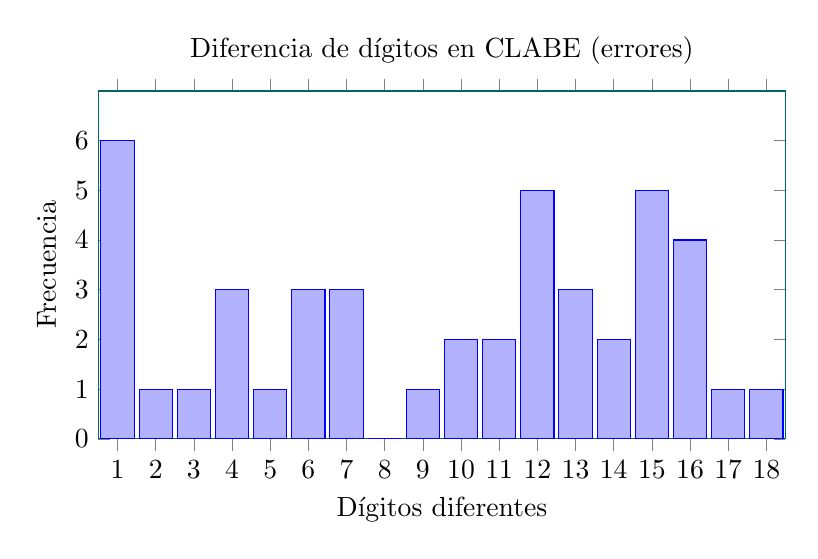
\begin{tikzpicture}
    \begin{axis}[
        ybar,
        bar width=12pt,
        width=0.85\linewidth,
        height=6cm,
        xlabel={Dígitos diferentes},
        ylabel={Frecuencia},
        ymin=0, ymax=7,
        xtick={1,2,3,4,5,6,7,8,9,10,11,12,13,14,15,16,17,18},
        xmin=0.5, xmax=18.5,
        ytick={0,1,2,3,4,5,6},
        fill=teal!60,
        draw=teal!80!black,
        title={Diferencia de dígitos en CLABE (errores)},
    ]
    \addplot coordinates {
        (1,6) (2,1) (3,1) (4,3) (5,1) (6,3) (7,3)
        (8,0) (9,1) (10,2) (11,2) (12,5) (13,3) (14,2) (15,5) (16,4) (17,1) (18,1)
    };
    \end{axis}
    \end{tikzpicture}
    \caption{Distribución de dígitos diferentes en CLABEs erróneas}
    \label{fig:clabe-digit-diff}
\end{figure}

Esta distinción resulta relevante porque sugiere dos tipos de intervención diferentes: los errores cercanos (1 a 7 dígitos) representan limitaciones de la capacidad de visión del modelo y difícilmente se resuelven con cambios de \textit{prompt}, mientras que los errores lejanos (10+ dígitos) corresponden a confusiones de campo que pueden mitigarse con instrucciones más específicas o con validaciones post-extracción.

\subsection{Rendimiento temporal y costo}

La Figura~\ref{fig:processing-time} muestra la distribución de tiempos de procesamiento por documento. La mediana fue de 1.9 segundos por archivo, con una media de 2.6 segundos y un máximo de 15.3 segundos. El 85\% de los archivos se procesaron en menos de 4 segundos; los valores atípicos corresponden a PDFs de múltiples páginas o documentos que activaron el mecanismo de \textit{retry}.

\begin{figure}[H]
    \centering
    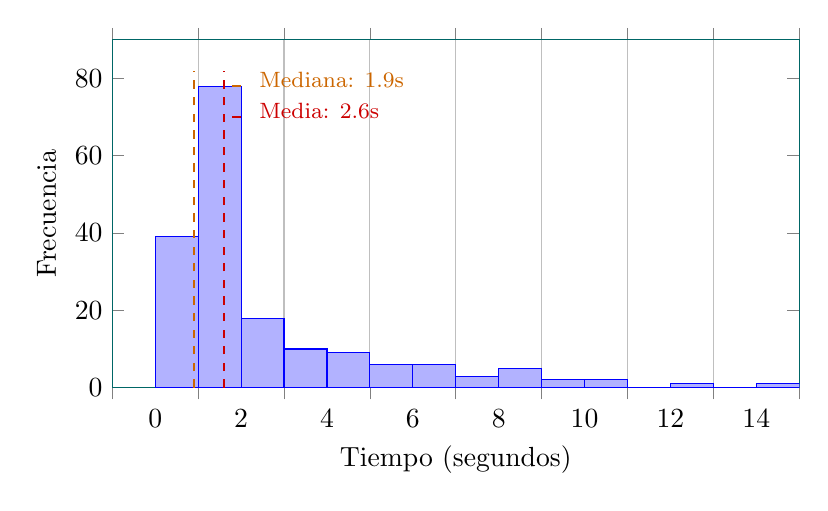
\begin{tikzpicture}
    \begin{axis}[
        ybar interval,
        bar width=12pt,
        width=0.85\linewidth,
        height=6cm,
        xlabel={Tiempo (segundos)},
        ylabel={Frecuencia},
        ymin=0, ymax=90,
        xmin=0, xmax=16,
        xtick={0,2,4,6,8,10,12,14,16},
        fill=teal!60,
        draw=teal!80!black,
    ]
    \addplot coordinates {
        (1,39) (2,78) (3,18) (4,10) (5,9) (6,6) (7,6)
        (8,3) (9,5) (10,2) (11,2) (12,0) (13,1) (14,0) (15,1) (16,0)
    };
    \draw[dashed, orange!80!black, thick] (axis cs:1.9,0) -- (axis cs:1.9,82);
    \draw[dashed, red!80!black, thick] (axis cs:2.6,0) -- (axis cs:2.6,82);
    \node[font=\footnotesize, anchor=south west, orange!80!black] at (axis cs:3.2,75) {Mediana: 1.9s};
    \node[font=\footnotesize, anchor=south west, red!80!black] at (axis cs:3.2,67) {Media: 2.6s};
    \draw[dashed, orange!80!black, thick] (axis cs:2.8,78) -- (axis cs:3.1,78);
    \draw[dashed, red!80!black, thick] (axis cs:2.8,70) -- (axis cs:3.1,70);
    \end{axis}
    \end{tikzpicture}
    \caption{Distribución de tiempos de procesamiento por documento}
    \label{fig:processing-time}
\end{figure}

La Tabla~\ref{tab:costos} resume el costo de procesamiento. El costo está dominado por los \textit{tokens} de entrada (98\% del total), ya que cada PDF se envía como documento binario completo codificado en base64, mientras que la respuesta estructurada es mínima. El costo promedio de \$0.011 USD por archivo resulta competitivo frente a servicios de OCR comerciales (típicamente \$0.01 a \$0.05 por página), con la ventaja de no requerir reglas de extracción manuales ni mantenimiento de plantillas por banco.

\begin{table}[H]
\centering
\vspace{6pt}
\begin{tabular}{lr}
\toprule
\textbf{Métrica} & \textbf{Valor} \\
\midrule
Precio input                          & \$1.00 USD / millón de tokens \\
Precio output                         & \$5.00 USD / millón de tokens \\
Tokens input promedio por archivo     & $\sim$13{,}500 \\
Tokens output promedio por archivo    & $\sim$100 \\
Costo promedio por archivo            & $\sim$\$0.011 USD \\
Costo total (176 archivos)            & $\sim$\$2.03 USD \\
Costo con \textit{retry} ($\sim$15\% archivos) & $\sim$\$2.20 USD \\
\bottomrule
\end{tabular}
\caption{Costo de procesamiento con Claude Haiku 4.5}
\label{tab:costos}
\end{table}

\subsection{Prompt de extracción}

El diseño del \textit{prompt} fue un factor determinante en la precisión alcanzada. A lo largo de la experimentación, el \textit{prompt} evolucionó desde una instrucción genérica de extracción hasta un conjunto de reglas específicas por campo, calibradas a partir del análisis de errores. La Tabla~\ref{tab:prompt-final} presenta las instrucciones clave del \textit{prompt} final.

\begin{table}[H]
\centering
\vspace{6pt}
\begin{tabular}{lp{10cm}}
\toprule
\textbf{Campo} & \textbf{Instrucciones principales} \\
\midrule
Titular & Buscar el nombre en la sección de datos del cliente. No confundir con el
nombre del asesor, ejecutivo, o personas mencionadas en transacciones. \\
CLABE & Distinguir explícitamente entre CLABE (18 dígitos), número de cuenta
(10--11 dígitos) y número de cliente (7--8 dígitos). Buscar el valor
inmediatamente al costado o debajo de etiquetas como ``CLABE'' o ``CLABE
Interbancaria''. Leer cada dígito individualmente. \\
Banco & Seleccionar de una lista cerrada de 12 instituciones financieras
mexicanas. \\
Validación & Si el documento no es un estado de cuenta bancario, marcar
\texttt{is\_valid\_document} como \texttt{false}. \\
\bottomrule
\end{tabular}
\caption{Instrucciones clave del \textit{prompt} de extracción final}
\label{tab:prompt-final}
\end{table}

El \textit{prompt} se complementa con un mecanismo de \textit{retry}: cuando la CLABE extraída no tiene exactamente 18 dígitos, se realiza una segunda llamada al modelo con instrucciones reforzadas que enfatizan la diferencia entre los campos numéricos. Si el \textit{retry} textual no produce un resultado válido y el documento es un PDF, se intenta adicionalmente una extracción sobre una versión rotada 90° de la primera página, lo cual resuelve casos de documentos con orientación incorrecta.


% =============================================================================
\subsection{Conclusiones experimentales}
% =============================================================================

Los resultados obtenidos permiten extraer tres conclusiones principales que fundamentan las decisiones de diseño del sistema. En primer lugar, el enfoque de envío directo de PDF al modelo demostró ser superior a todas las alternativas evaluadas, tanto en precisión como en simplicidad de la arquitectura. Cuando se eliminan las etapas intermedias de OCR o conversión a imagen, se reduce la superficie de error y se simplifica el mantenimiento del sistema. La mejora más significativa se observó en el campo Banco (de 41.5\% a 96.6\%), confirmando que el acceso simultáneo a contenido textual y visual es fundamental para documentos donde la información clave aparece como logotipo o elemento gráfico. En segundo lugar, el análisis de errores reveló que la precisión de la extracción depende fuertemente del diseño del \textit{prompt} y de las instrucciones específicas por campo. El \textit{prompt} genérico inicial alcanzó 80.8\% en CLABE; tras incorporar instrucciones de desambiguación entre campos numéricos e indicaciones de ubicación espacial, la precisión subió a 90.9\%. Sin embargo, ciertos formatos bancarios (como BanBajío) resistieron todas las mejoras de \textit{prompt} intentadas, lo que evidencia que existen límites inherentes a lo que puede resolverse únicamente mediante instrucciones textuales cuando el diseño visual del documento genera ambigüedad entre campos. En tercer lugar, la variabilidad de resultados por banco, desde 0\% en CLABE para BanBajío hasta 100\% para HSBC, demuestra que no existe un \textit{prompt} universal óptimo para todos los formatos de documentos. Esta observación motivó la decisión de implementar un sistema de extractores configurables, donde cada usuario puede definir su propio \textit{prompt}, esquema de salida y modelo según las características de sus documentos. En lugar de intentar construir un extractor monolítico que cubra todos los casos, el sistema delega la especialización al usuario, proporcionando herramientas de asistencia, generación de esquemas y \textit{prompts} con IA, y mecanismos de evaluación (extracciones de prueba con resultados visibles) para facilitar la iteración. De esta manera, los hallazgos experimentales no solo validan la viabilidad técnica del enfoque, sino que informan directamente la arquitectura del producto final.
